\documentclass[a4paper]{jlreq}

% 数式
\usepackage{amsmath,amssymb,bm}

% 図表
\usepackage{graphicx}
\usepackage{booktabs}

% 化学式・単位
\usepackage[version=4]{mhchem}
\usepackage{siunitx}

\title{情報レポート～二十四節気表示UIの提案～}
\author{学籍番号: J4-260535 川合敦己}
\date{\today}

\begin{document}

\maketitle

このレポートや Python コード、および Web アプリケーション \texttt{solar-calendar} のソースコードは、
以下の GitHub リポジトリにて公開している。
\par
https://github.com/kawaii-kawai/20260507\_Informatics
\par
https://github.com/kawaii-kawai/solar-calendar

\section*{Q1}

教科書 pp.~96--102 に記されたアルゴリズムは、 $m$ 月 $d$ 日から $n$ 日後の日付を求めるために、
擬似的に $m$ 月 $d+n$ 日を計算し、その後 $d+n$ が $m$ 月の日数を超える場合は、
$m$ を 1 増やし、 $d+n$ から $m$ 月の日数を引くことを繰り返すものである。
実際、立春から八十八夜の日付を求める際に年をまたぐことはなく、このアルゴリズムは正当である。
ただし、今回は一般的な日付計算にも対応させるため、西暦 1 年 1 月 1 日からの経過日数に変換して
年月日を計算する方法を採用した。
この際の処理は基本的に同様であるが、グレゴリオ暦の閏年規則を考慮するため、実装はやや複雑になる。

以下に実行例を示す。

\begin{verbatim}
(.venv) kawaiatsuki@Riko:~/dev/Informatics/0507$ python 01.py 2026 2 4 87
2026 5 2
\end{verbatim}

\section*{Q2}

このプログラムを改良することを考える。問題点は以下の通りである。

\begin{itemize}
    \item ユーザーを想定したソフトウェアとして考えたとき、CUI での入力はユーザーフレンドリーとは言い難い。
    \item 八十八夜の日付を知らないユーザーが、立春の日付を知っているとは限らない。
    \item 八十八夜だけに関心を持つユーザーは限定的である。
\end{itemize}

これらを解決するため、Web アプリケーションとして二十四節気と八十八夜を視覚的に表示する
\texttt{solar-calendar} を作成した。公開先は次の通りである。
\par
https://kawaii-kawai.github.io/solar-calendar/
ただし、スマートフォンでの利用のみを想定しており、またブラウザによっては正常に動作しない可能性がある。

具体的には以下の機能を持たせた。

\begin{itemize}
    \item 二十四節気を円周上に配置し、地球を模したオブジェクトを回転させて操作する。
    \item 地球の公転を模した回転により、年を切り替える。
\end{itemize}

本ソフトウェアは、二十四節気や八十八夜に詳しくない(自分のような)現代人をユーザーを想定している。
二十四節気が地球の公転による太陽との位置関係の変化で決まることを視覚的に理解でき、
操作を公転に見立てることで直感的な操作を可能にした。
また、節気の簡単な説明とふりがなを表示し、二十四節気や八十八夜に対する理解を助けることも目指した。

\subsection*{システム概要}

ブラウザ上で動作する二十四節気表示ソフトウェア \texttt{solar-calendar} を TypeScript と React で開発した。
UI は SVG で描画し、GitHub Pages にホスティングした。
ドラッグ操作で地球オブジェクトを回転させ、年を切り替える。
二十四節気のデータは外部から取得した \texttt{public/data/sekki.json} を使用し、
さらに、立春から数えて 88 日目の八十八夜を自動計算し、円周の外側に控えめに表示した。
なお、実装には GPT-5.2-Codex を用いて、UI 部分のコーディング支援とリファクタリングを行った。

\begin{figure}[tb]
    \centering
    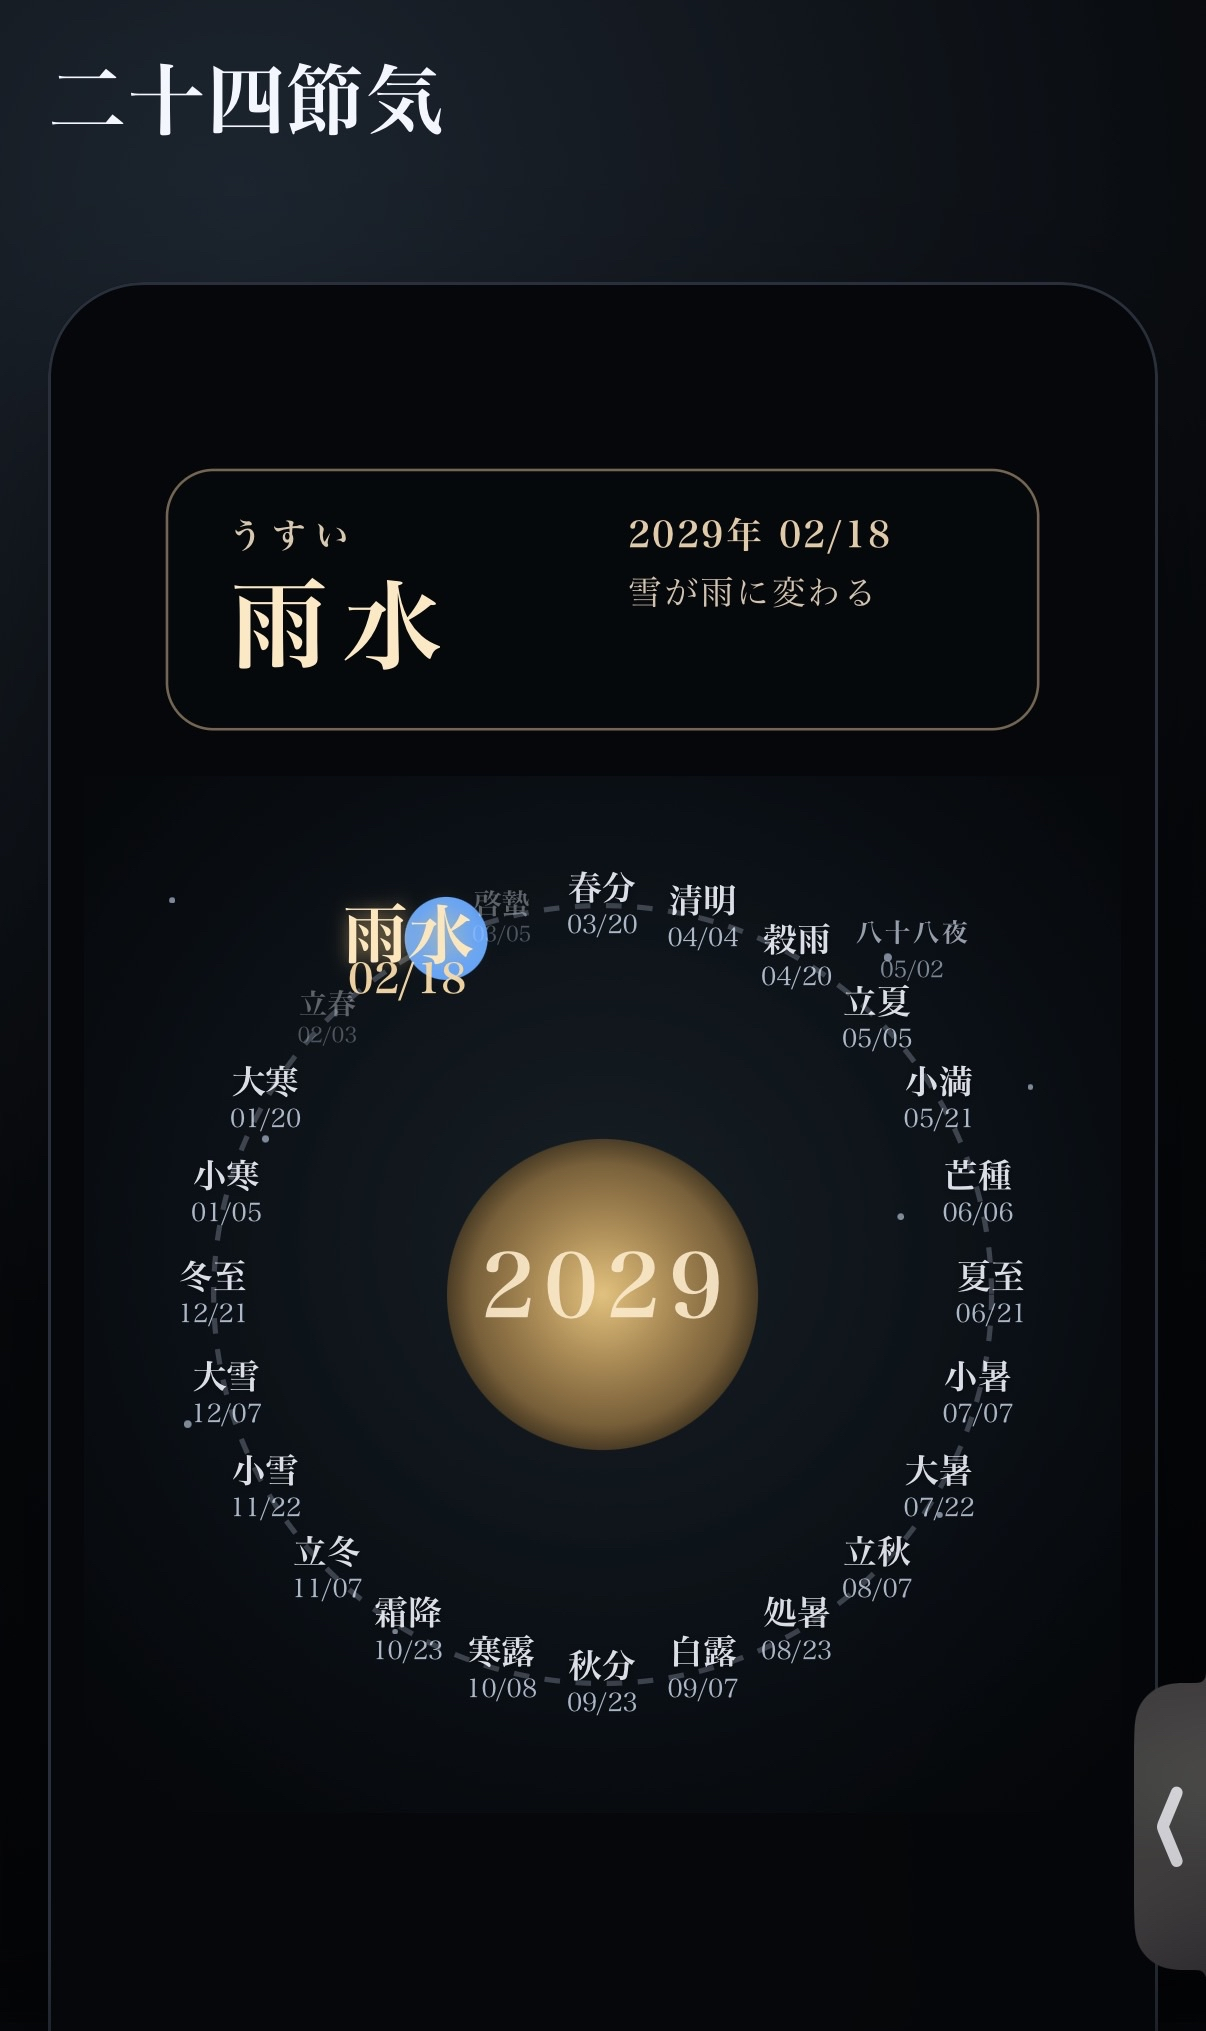
\includegraphics[width=0.8\linewidth]{IMG_0203.png}
    \caption{スマートフォンでの表示例1}
\end{figure}

\begin{figure}[tb]
    \centering
    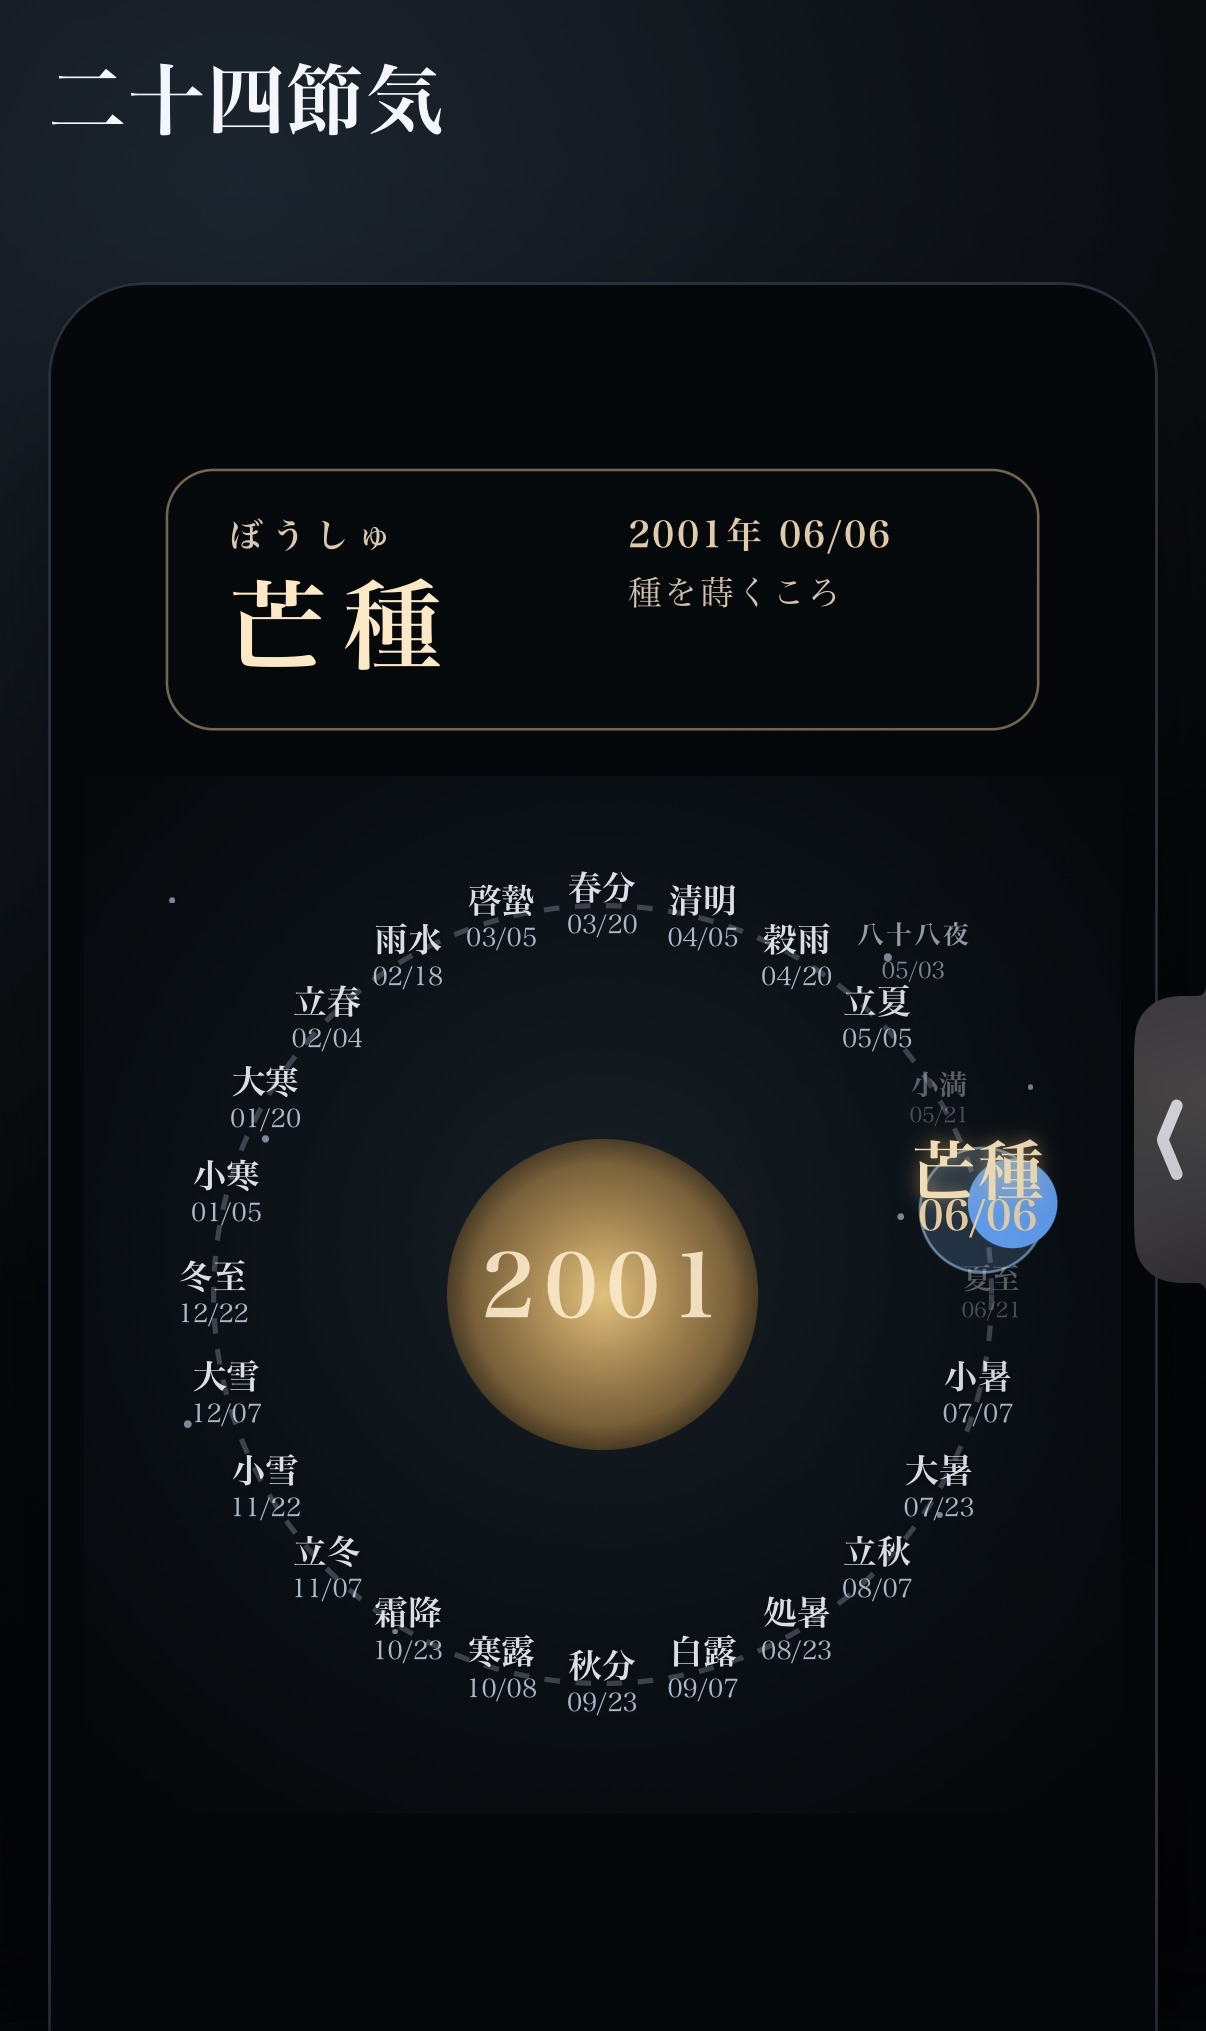
\includegraphics[width=0.8\linewidth]{IMG_0204.png}
    \caption{スマートフォンでの表示例2}
\end{figure}

\subsection*{成果}

\begin{itemize}
    \item 二十四節気を円周上に配置し、位置関係を直感的に理解できる。
    \item 慣性付きのドラッグ操作により、滑らかな年切替を実現した。
    \item 強調表示により、現在の節気と日付が一目で分かる。
    \item 八十八夜を自動計算し、補助情報として表示できた。
\end{itemize}

\subsection*{問題点と展望}

今回作成した \texttt{solar-calendar} には、以下のような問題点がある。

\begin{itemize}
    \item 動きのある UI に対し、二十四節気の日付は毎年ほぼ同じで変化が少ない。
    \item 年の切替が冬至と小寒の間で起きるため、年の変化を実感しにくい。
    \item iPodのクイックホイールのような直感的な操作感を目指したが、ドラッグの触感は改良の余地がある。
    \item 外部データに欠損があり、年の範囲も 2000 年から 2030 年までに限定される。
\end{itemize}

これらの問題点を解決するために以下のような改良が考えられる。

\begin{itemize}
    \item 二十四節気の日付が変わるタイミングで、地球オブジェクトの周りにエフェクトを表示するなどして、ユーザーが年の切り替わりを実感できるようにする。
    \item あるいは、すべての二十四節気に対して通過したタイミングで次の年に切り替えるなど、即応性の高く、変化のわかりやすい UI にする
    \item 二十四節気のデータを天体計算に基づいたものにしたり、国立天文台の Web ページからスクレイピングするなどして、より正確で、長期間のデータを用いる。
\end{itemize}

なお、二十四節気のデータに関しては、Python の天体計算ライブラリ \texttt{skyfield} を用いた計算も試みたが、
実際の節気日付とは数日程度のずれが生じた。
また、国立天文台が公開している二十四節気のデータは現時点で 2027 年までに限られ、
スクレイピング対象ページの構造も複雑であるため、本レポートでは外部データを用いた。

\end{document}
